\chapter{Related work}
\label{c:relatedwork}

\todo[inline]{Introductory Paragraph}
\todo[inline]{Structuring}

\begin{figure}[b]
	\centering
	
	\begin{subfigure}[b]{0.45\textwidth}
		\centering
        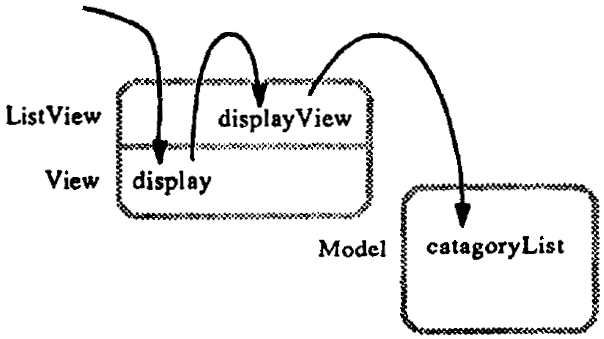
\includegraphics[width=\textwidth]{../images/06-Cunningham-Diagram}
        \caption[Foo]{}
		\label{fig:06-1-Cunningham}
	\end{subfigure}
	\quad
	\begin{subfigure}[b]{0.45\textwidth}
		\centering
		
\includegraphics[width=\textwidth,height=2cm]{../images/foo}
		\caption[Bar]{}
		\label{fig:06-1-Foo}
	\end{subfigure}
	
	\caption[TOC Caption]{
		a) Cunningham's and Beck's notion of diagramming object interactions, taken from \cite{cunningham_diagram_1986}.
		b) ...
	}
	\label{fig:06-1}
\end{figure}

Cunningham and Beck propose a syntax for diagramming the message sending dialogue between objects in object-oriented computations (see Figure \ref{fig:06-1-Cunningham}) \cite{cunningham_diagram_1986, beck_system_1989}.
Similar to \textsc{PathObjects}, objects are drawn as boxes and message sends are represented by directed arcs between them.
Unlike the notation used by \textsc{PathObjects}, the space inside the boxes is not used to model the object state, but to emphasize method overrides and calls to implementations of superclasses.
For that purpose, the class hierarchy is represented by layers in a box.
Since the authors regard overriding as the more important concept over inheritance, subclasses are placed above superclasses in these layers. 
To allow for the generation of such diagrams, an additional pane is added to the Smalltalk-80 debugger. 
Objects and messages are added to this diagram area when using the standard debugger commands \emph{step} and \emph{send}. 
However, as automatic layouting is not supported, objects have to be placed by the user manually. 
The authors state that the debugger extension helped them to understand complicated computations better, enabling them to fix a long standing bug in the Smalltalk core.

Lange and Nakamura present \textsc{Program Explorer} in the context of design pattern based framework understanding \cite{lange_interactive_1995, lange_program_1995}.
Based on the assumption that the combination of abstract concepts like classes and their relationships and the concrete objects and their interactions is the fundamental requirement to the understanding of object oriented systems, \textsc{Program Explorer} offers class inheritance views, object graphs and interaction charts.
Contrary to our approach, object state exploration is not supported.
To ensure a certain degree of scalability of the information presentation, \emph{view navigation} and \emph{integration} are provided.
Within a given view, \emph{navigation} can be used to explore the presented information interactively, starting from an initial focus point and going to regions of further interest.
\emph{Integration} enables the user to transfer a defined focus between different views.
Both concepts are similar to the navigation through a scenario offered by \textsc{PathObjects} and the bidirectional connection to the static view provided by \textsc{PathView}.
To reduce the size of the traces that are generated from instrumented executions of C++ programs, \textsc{Program Explorer} also supports \emph{trace localization}, which means that classes of interest can be selected through the instrumentation GUI and only selected classes will be instrumented.
As compared to \textsc{PathObjects}, the latter offers a more fine-grained approach through the selection of methods of interest, instead of solely filtering by classes.

\textsc{Collaboration Browser} by Richner and Ducasse \cite{richner_using_2002} is a tool that focuses on the recovery of object collaborations and roles from dynamic information.
Since the process of automatic design recovery is said to yield poor results, the authors favor an iterative process steered by an engineer.
To facilitate such a process, \textsc{Collaboration Browser} offers two main features: \emph{pattern matching} and \emph{querying}. 
Typically, a user would first create collaboration patterns by defining pattern matching criteria, and then proceed by iteratively querying about patterns in which classes or methods of interest participate.
Finally, to understand a collaboration, an instance of a collaboration pattern can be visualized in the form of interaction diagrams, which are almost identical to UML sequence diagrams. \todo{compare to PathObjects}

Systä et al. present a reverse engineering environment called \textsc{Shimba} \cite{systa_shimba_2001}, which supports both static and dynamic analysis of Java software systems.
Static information about software entities like classes, interfaces and their relationships is extracted from the bytecode representation and visualized using \textsc{Rigi} \cite{muller_understanding_1993} in the form of directed dependency graphs.
Besides the computation of some of the metrics of Chidamber's and Kemerer's suite \cite{chidamber_metrics_1994}, \textsc{Rigi} also can be utilized to build abstractions, for instance by aggregating classes into their respective packages.
Runtime traces are collected with the help of a customized SDK debugger and can be synthesized as UML-like sequence and statechart diagrams through \textsc{SCED} \cite{koskimies_automated_1998,systa_understanding_2000}.
\textsc{Shimba} supports bidirectional model slicing between \textsc{Rigi} graphs and \textsc{SCED} diagrams.
On one side, \textsc{Rigi} can be used to restrict the amount of collected execution events through the selection of components of interest. Thus, the scope of the generated \textsc{SCED} diagrams is reduced.
On the other side, starting from a \textsc{SCED} diagram, static views covering the affected components can be obtained.